\documentclass[a4paper, 10pt, twoside, openright]{report}
\usepackage[top=2cm, bottom=2.5cm, left=2.5cm, right=2.5cm]{geometry}
\usepackage{graphicx}
\usepackage{booktabs}
\usepackage{url}
\usepackage[english]{babel}
\usepackage[latin1]{inputenc}
\usepackage{hyperref}
\hypersetup{
    colorlinks,
    citecolor=black,
    filecolor=black,
    linkcolor=black,
    urlcolor=black
}
\usepackage{mathenv}
\usepackage{amsmath}
\usepackage{mathtools}
\usepackage{color}
\usepackage{caption}
\usepackage[bottom]{footmisc}
\usepackage{cancel}
\usepackage{multirow}
\usepackage[toc,page]{appendix}
\usepackage[]{acronym}
\usepackage{setspace}
%\usepackage[Sonny]{fncychap}
\usepackage{fancyhdr}
\usepackage{titlesec}
\usepackage{gensymb}
\usepackage{emptypage}

\makeatletter
\titleformat{\chapter}[block]
  {\Huge}{\filright\enspace \@chapapp~\thechapter\enspace \\}
  {8pt}{\Huge\bfseries\filcenter}
\titlespacing*{\chapter}
  {0pt}{0pt}{20pt}
\makeatother

%\setlength{\headheight}{20pt}
%\pagestyle{fancy}
%\renewcommand{\chaptermark}[1]{\markboth{#1}{#1}}
%\rhead{\thepage \hfill \leftmark}
%\lhead{\thepage \hfill \leftmark}
%\cfoot{}

\begin{document}

\renewcommand{\listfigurename}{List of figures} 
\renewcommand{\listtablename}{List of tables}

%Titlepage
\doublespacing
\baselineskip=0.8\baselineskip
\setlength{\parindent}{0pt}	

\pagenumbering{roman}
\begin{titlepage}

	\centering
	
\includegraphics[width=0.15\textwidth]{figs/image_UC.png}\par
	{\scshape\LARGE Facultad de Ciencias \\ \vspace{-15pt} Universidad de Cantabria \par}
	
	\vspace{0.8cm}
	
	%English title
	\noindent\rule{15cm}{0.4pt}\par 
	{\huge\bfseries Search for dark matter production in association with top quarks in the dilepton final state at $\sqrt{s} = $ 13 TeV\par}
	\noindent\rule{15cm}{0.4pt}\par 
	
	{\vspace{20pt} \Large A thesis submitted in fulfillment of the requirements for the \par \LARGE \textbf{Degree of Doctor of Philosophy} \vspace{20pt} \par \noindent\rule{15cm}{0.4pt}}
	
	\vspace{1.2cm}
	{\Large Written by \\ \textbf{C�dric Prie�ls}\par}
	\vspace{1.0cm}
	{\Large Under the supervision of \\ \textbf{J�natan Piedra G�mez} \\
	\textbf{Pablo Mart�nez Ruiz del �rbol}\\}
	\vspace{2cm}
	{\Large June 2020}
	\vfill

\end{titlepage}

%Empty page

%\clearpage
%\thispagestyle{empty}
%\phantom{a}
%\vfill
%\newpage

%Abstract and keywords

\setcounter{page}{1}

\chapter*{\huge{Abstract}}
\newpage
%
\chapter*{\huge{Resumen}}
\newpage
%
\chapter*{\huge{Acknowledgements}}
\newpage
%
\chapter*{\huge{Acronyms used}}
\begin{acronym}

%List all the acronyms used
\acro{SM}[SM]{Standard Model}
\acro{DM}[DM]{Dark Matter}
\acro{LHC}[LHC]{Large Hadron Collider}
\acro{CMS}[CMS]{Compact Muon Solenoid}
\acro{ATLAS}[ATLAS]{A Toroidal LHC ApparatuS}
\acro{CERN}[CERN]{European Council for Nuclear Research}
\acro{CMB}[CMB]{Cosmic Microwave Background}
\acro{ML}[ML]{Machine Learning}
\acro{MFV}[MFV]{Minimal Flavour Violation}
\acro{WIMP}[WIMP]{Weakly Interactive Massive Particles}
\acro{PF}[PF]{Particle Flow}
\acro{BSM}[BSM]{Beyond the Standard Model}

\end{acronym}
\newpage

%Table of contents
\tableofcontents

\thispagestyle{empty}
\newpage

%Here it starts!
\setlength{\parskip}{10pt}
\pagenumbering{arabic}

%Introduction

\chapter{Introduction}

The \ac{SM} of particle physics is nowadays the most accepted mathematical model used to describe the elementary particles and three of the four fundamental forces of nature (electromagnetic, weak and strong interactions). This model is quite simple in concept, but has been able to describe most of the phenomena observed in nature so far with an incredible level of precision, and made a lot of predictions that have now been proven to be true, such as the postulate of the Higgs mechanism \cite{HiggsPostulate1, HiggsPostulate2} followed by the discovery of the Higgs boson itself in 2012 \cite{HiggsDiscovery1, HiggsDiscovery2} by the \ac{CMS} and \ac{ATLAS} experiments of the \ac{CERN}. 

However, as accurate as it seems to be, this theory is known to have several shortcomings which require further investigation. Eventual exotic particles which do not fit in the current model could be the sign of new physics and have therefore been extensively searched for over the course of the last decades in order to enhance our understanding of the Universe and all its constituents.

In this context, the first serious \ac{DM} hypothesis was introduced in the 1970s because of gravitational anomalies observed by several astrophysicists, as a way to explain the apparent non-luminous missing mass in the Universe \cite{FirstEvidence}. Indeed, the visible mass in most galaxies appears to be way too low to explain several astrophysical processes, such as the rotation curves of the galaxies \cite{RotationCurves}, which seems to be incompatible with the well established laws of gravitation. Some additional measurements of the gravitational lensing (in the Bullet Cluster, for example \cite{BulletCluster}) and the anisotropies observed in the \ac{CMB} \cite{CMBAnisotropies} can be quoted among other evidences for the existence of \ac{DM}, as explained in details in Section~\ref{section:DMOrigins}.

As far as we currently know from cosmological measurements, ordinary baryonic matter only constitutes around 5\% of the Universe, while  \ac{DM} represents around 26\% of the energy density of the Universe (the rest is being considered as dark energy) \cite{Repartition}. Understanding the nature and properties of this new kind of exotic matter is therefore crucial to try and understand the physics in the Universe. 

Nowadays, the existence of \ac{DM} is well established in the physics community, even though it has never been observed directly, since our only evidences so far for its existence come from its large-scale gravitational effects. While its nature is still unknown and extensively studied, one of the best \ac{DM} candidate is the so-called \ac{WIMP}s, predicted to interact both gravitationnaly and weakly with \ac{SM} particles. This would allow direct and indirect direction of such candidates, used as the driving process of many of experiments over the last decades, trying to find the hint of a possible interaction between standard baryonic particles and eventual \ac{DM} particles, or even between several \ac{DM} particles themselves. Dark matter production through the use of a particle accelerator colliding \ac{SM} particles together, such as the \ac{LHC}, is also a possibility, and will be consider as the main channel towards the eventual detection of this exotic matter throughout this work. The production through colliders is actually able to provide constraints on low dark matter masses as well, in a region where both the direct and indirect searches are less efficient, which makes the \ac{LHC} a perfect tool to study this kind of \ac{BSM} physics. 

However, observing \ac{DM} is still extremely difficult, mainly because it barely interacts with ordinary baryonic matter, except through gravity (we have to assume that it does interact with \ac{SM} at least weakly for the sake of this work though, as we would not be able to discover it as an individual particle if it were not the case). This means that nowadays, all the experiments searching for \ac{DM} have only been able to put constraints on the \ac{DM} particle mass and on the interaction cross sections between the dark and standard sectors. Actually, even if the collisions between protons produced by the LHC do have an sufficient amount of energy to produce this kind of particles, we would not expect them to interact with our detector, meaning that a direct detection is out of our hands for now. The eventual presence of such matter has to be inferred from the study of the interaction between \ac{SM} particles and \ac{CMS} itself, since a typical \ac{DM}-like event consists of at least one energetic \ac{SM} particle produced in association with a large imbalance in the transverse momentum due to the presence of an eventual \ac{DM} candidate that was able to escape our detection. %This kind of collider searches can be grouped under the name of \textit{mono-X} searches, where the \textit{X} stands for any kind of \ac{SM} particle (a jet, a lepton or a photon for example). 

In the context of this work, \ac{DM} is searched for in association with one or two top quarks which play the role of the \ac{SM} particle allowing us to trigger the event. This is indeed a perfect channel for this kind of searches if we assume that the interaction between the dark and standard sectors respect the principle of \ac{MFV}, which can be consistently defined independently of the structure of the new physics model \cite{MFVYukawa}. In this case, this interaction should follow the same Higgs-like Yukawa coupling structure as the usual \ac{SM} baryonic particles. This is an important consequence, since it will be shown in Section~\ref{section:DMProperties} that this coupling is actually stronger with more massive particles: the heavier the \ac{SM} particle considered is, the easier it is for this particle to couple with the dark sector. This makes the top quark, the most massive of all the fundamental particles observed by far, is therefore an excellent object to study in this context.

However, this also means that its phenomenology is mostly driven by its large mass and that it decays before hadronization can occur, usually into a W boson and and a bottom quark ($\sim$96\% branching ratio \cite{PDG}). The final state of the process we are interested in is then be made out of some b jets, leptons and/or quarks and is be categorized depending on this number of b jets and on the decay of the W itself. This work will actually be focused on the two leptons final state, also known as the dileptonic channel, mostly since this channel does not have lots of background processes raising to a similar final state, even though its branching ratio is the smallest, as will be explained in Section~\ref{section:ourChannel}. Additionally, leptons are by reconstruction much cleaner than jets. This means that their identification and momentum calculation is easier to perform, and that the uncertainties associated to these measurements will be smaller.

The LHC has now been running for 10 years, and several similar searches have already been carried out and published in the past by the CMS and ATLAS collaborations, at different center of mass energies. First of all, at 8 TeV, several searches for a pair of top quarks were published by the CMS (in association with \ac{DM} in the semileptonic \cite{PreviousDoubleTopSingleLep8CMS} and dileptonic \cite{PreviousDoubleTopDiLep8CMS} final states) and ATLAS collaborations \cite{PreviousDoubleTopAllLep8ATLAS}. At 13 TeV, the ATLAS collaboration published on one hand several studies, considering different final states \cite{PreviousDoubleTopNoLep13ATLAS, PreviousDoubleTopOneLep13ATLAS, PreviousDoubleTopDiLep13ATLAS}. On the other hand, the CMS collaboration published a few extremely important papers for this study \cite{PreviousDoubleTopBottomAllLep13CMS, PreviousDoubleTopAllLep13CMS}. For the first time in 2019, the results obtained by the single top and $t \bar t$ analyses have also been combined and published using the 2016 data \cite{PreviousSingleDoubleTopAllLep13CMS}. Our main objective is now to repeat and improve this analysis that was performed while considering a larger dataset, globally improving the analysis strategy and including the dileptonic final state for the first time in this combination.

After a detailed introduction about \ac{DM} in general, the experimental device will be detailed in the Chapter~\ref{chapter:Device}. This will include a discussion about the \ac{LHC} itself, along with a complete description of \ac{CMS}, the detector used to collect the data that will be analyzed throughout this work. This data has been collected during the years 2016, 2017 and 2018 and corresponds to an integrated luminosity of $\sim 138$ fb$^{-1}$, collected during the Run II of operation of the \ac{LHC} and at a center of mass energy $\sqrt{s} = 13$ TeV. In particular, a particular care will be given to the explanation of the \ac{PF} algorithm, used to reconstruct the different objects used and that will be defined in the Chapter~\ref{chapter:Reco}, while the estimation of the different backgrounds and the selection of interesting events will be detailed throughout the Chapters~\ref{chapter:Samples} and ~\ref{chapter:Selection}.

Distinguishing between the signal we are searching for and backgrounds having a much higher cross-section and kinematically really close, such as the \ac{SM} $t \bar t$ without production of \ac{DM} is not a straightforward task (sometimes a production of missing transverse energy due to the presence of physical neutrinos is even obtained). To isolate the signal and to obtain some discrimination between these kind of processes, an algebraic reconstruction of the event and top-notch \ac{ML} techniques are used in this work, in order to train a network of neurons. The main objective is to make them learn how to combine the discriminating power of a set of input variables in order to create a single output variable describing the probability of a single event to be classified as signal or background. All this process will be detailed in Section~\ref{section:Discrimination}.

Finally, a statistical interpretation of our data will be performed and different sources of systematic uncertainties will be considered in the Chapter~\ref{chapter:FinalResults}. This will allow us to set upper limits on the cross section production value of \ac{DM} particles in our particular channel and for the simplified models considered in this analysis. The conclusions of this work and some additional future prospects will then finally be presented in Chapter~\ref{chapter:Conclusion}.
\\

%Empty page

%\clearpage
%\thispagestyle{empty}
%\phantom{a}
%\vfill
%\newpage

\chapter{The Dark Matter case}

In this chapter the case for \acf{DM} will first of all be presented in Section~\ref{section:DMOrigins}, along with a summary of the main evidences, mostly astrophysical, which lead to the introduction of this kind of \acf{BSM} physics. Then, the main properties expected by such exotic matter will be introduced in Section~\ref{section:DMProperties} and nowadays's most accepted \ac{DM} candidates, such as the \acf{WIMP} briefly introduced previously will be presented in Section~\ref{section:DMCandidates}. The main ways we have to search for this new physics will then be shown in Section~\ref{section:DMSearches}. 

Finally, the searches performed in colliders such as the \acf{LHC} and our particular channels of interest (\ac{DM} produced in association with either one or two top quarks) will be detailed in Section~\ref{section:ourChannel} and the latest similar results and exclusion plots published over the course of the previous years by the ATLAS and CMS collaborations will be shown in Section~\ref{section:PreviousResults}.

\section{At the origins of dark matter} \label{section:DMOrigins}

The origin of the concept of dark matter can be traced back to the 17 and 18th centuries, shortly after Newton's works on gravitation, even though this concept changed a lot over the years. Back then, \ac{DM} was more considered to be ordinary matter which simply did not emit any kind of electromagnetic radiation, being therefore invisible and dark, but which does have a strong impact in the gravitational point of view because of its mass. It was for example considered in the 20th century to be found in massive astronomical objects able to absorb the light or other objects located behind them, such as black holes.

\subsection{Zwicky and the virial theorem}

Around this time, the first experimental evidences for the existence of dark matter were shown. In 1933, Fritz Zwicky managed to determine the mass of the Coma Cluster using the virial theorem \cite{Zwicky}, which states that if in a cluster in equilibrium under its own gravitation, the kinetic energy must be comparable to the gravitational binding energy. 

Mathematically, the virial theorem can be written in Equation~\ref{equation:Virial}, where the brackets represents the mean value of the quantity obtained over time or position, the universal constants of gravitation $G = 6.67 \cdot 10^{-11}$ m$^3$ kg$^{-1}$ s$^{-2}$ and where the gravitation potential energy expression can be simplified assuming a spherical distribution of the masses and the same average density everywhere in the cluster.

\begin{equation} \label{equation:Virial}
2 \langle T \rangle + \langle V \rangle = 0 \text{, where}
\begin{dcases}
T = \frac{1}{2} \sum_i M_i v_i^2 = \frac{1}{2} M \langle v^2 \rangle\\
V = -4 \pi G \int_0^R M \rho r dr \propto \frac{G M^2}{R}
\end{dcases}
\end{equation}

Solving these simple equations gives us an approximate value of the mass of the cluster in Equation~\ref{equation:ClusterMass}, where R is the radius of the cluster and $\langle v^2 \rangle$ is the squared velocity of all the galaxies averaged over time.

\begin{equation} \label{equation:ClusterMass}
M \propto \frac{\langle \langle v^2 \rangle \rangle R}{G}
\end{equation} 

From this simple expression and astronomical observations, Zwicky then managed to compute the average mass to light ratio of its galaxies and concluded that the value obtained was around 500 times larger than the mass previously estimated by Edwin Hubble, who simply considered the number of visible galaxies within this cluster. One plausible explanation for this discrepancy is to introduce the concept dark matter, which contributes to the mass of the cluster without increasing the galactic luminosity.

Zwicky's results were actually quite controversial since they were based on statistical calculations relying on different hypotheses not always justified, such as the fact that the galaxies in the cluster must be gravitationnaly bound with each other and they were actually proven to be overestimated later on \cite{ZwickyWrong}.

\subsection{Spiral galaxies rotation curves}

Despite being controversial and slightly off, Zwicky's results were soon followed by a series of additional astronomical observations leading to the same conclusion, the possible existence of non-luminous matter in all the galaxies, called dark matter. The most famous of these results is the study of the observed and expected rotation curves of the stars within spiral galaxies such as the Milky Way in the 1970s \cite{RotationCurves}. 

According to this study, if we assume that we can apply Newton's universal laws of gravitation at the galactic scale, then the stars within this kind of galaxies should rotate with a velocity depending on the radius to the galactic center obtained by the usual equation for centripetal acceleration in a gravitational field and represented in Equation~\ref{equation:RotationVelocity}, where $M(r)$ accounts for the total mass encountered within a radius $r$.

\begin{equation} \label{equation:RotationVelocity}
v_{\text{rotation}}(r) = \sqrt{\frac{G M(r)}{r}}
\end{equation}

At first approximation, one can assume that most of the most within this kind of galaxies comes from the inner core, meaning that, at large radius, the velocity of individual stars is expected to decrease proportionally to $r^{-1/2}$. 

However, observations made by Vera Rubin and her team in the early 1970s with a new spectrograph designed the velocity curves of spiral galaxies with a degree of accuracy never reached before, did not confirm these expectations \cite{VeraRubin}. Indeed, according to these results, from a given value of the radius, the velocity curve appears to be flat instead of decreasing as expected, as illustrated in Figure~\ref{figure:RotationCurves}.

\begin{figure}[htbp]
\begin{center}
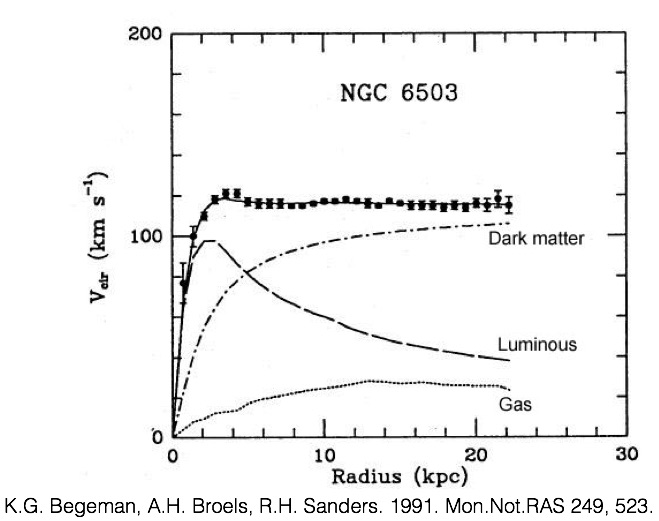
\includegraphics[width=8cm, height=6cm]{figs/RotationCurve.jpeg}
\caption{Expected and observed rotation curves of the galaxy NGC 6503 \cite{RotationCurves}. The black dots correspond to the data and the \textit{luminous} line corresponds to the expected rotation curve.}
\label{figure:RotationCurves}
\end{center}
\end{figure}

\vspace{-10pt}
\subsection{\acf{CMB} anisotropies} \label{subsection:CMB}

The \ac{CMB} is a mostly uniform background of primary radio waves emitted when the Universe became transparent around 380.000 years after the Big Bang and was discovered accidentally in the 1940s \cite{CMBDiscovery}. Studying it is extremely important, as it is actually made out of the oldest and cleanest electromagnetic radiation we can find in the Universe. Precise measurements of this radiation are actually critical in many different fields of physics, since any proposed model of the Universe must be able to explain this radiation, its temperature and anisotropies. 

Recent measurements determined that the \ac{CMB} can be considered as emitting a thermal black body spectrum at a temperature of $(2.72548\pm 0.00057)$K \cite{CMBTemperature}. However, we now know that this temperature is actually not constant as some small anisotropies (at the $10^{-5}$ level) depending on the value of the angular angle of observation can be observed. 

We see these fluctuations projected over a 2D sphere, and it is therefore natural to introduce at this point Laplace's spherical harmonics, $Y_{lm} (\theta, \phi)$, a complete set of orthogonal functions defined on a sphere and defined by a few parameters such as $l$, the multipole, representing a given angular angle in the sky (l=100 corresponds to $\sim 1\degree$) and $m$, the number of poles, such as $-l \leq m \leq l$ \cite{PowerSpectrum}. 

The temperature fluctuations, whose value depend on the two usual spherical angles $\theta$ and $\phi$ can then be expanded using these generic functions, according to Equation~\ref{equation:SphericalHarmonics}.

\begin{equation} \label{equation:SphericalHarmonics}
\frac{\Delta T}{T}(\theta, \phi) = \sum_{l, m} a_{lm} Y_{lm} (\theta, \phi)
\end{equation}

The information about the anisotropies can actually be extracted from the values of the $a_{lm}$ coefficients, from which we can obtain the values needed to represent the power spectrum of the \ac{CMB}, according to Equation~\ref{equation:PowerSpectrum}, and from which most of the cosmological information of the \ac{CMB} can actually be derived.

\begin{equation} \label{equation:PowerSpectrum}
D_l = \frac{l(l-1) C_l} {2\pi} = \sum_m |a_{lm}^2|
\end{equation}

Interestingly enough, this spectrum is directly affected by the value of the density of the dark matter in the Universe. Doing a multi-parameters fit on the observed data in this plot is then able to give us directly the energy density of baryonic $\Omega_b$ and dark $\Omega_\chi$ matter, along with other important parameters of the $\Lambda CDM$ cosmological model. Today's most precise measurements have been obtained in 2018 using the Plank satellite, and lead to the determination of these two quantities: $\Omega_b h^2 = 0.02220 \pm 0.00020$ and $\Omega_\chi h^2 = 0.1185 \pm 0.0015$ \cite{Planck} and the actual power spectrum obtained represented in Figure~\ref{figure:CMBSpectrum}.

By dividing these results with the value of the scaling factor for Hubble expansion rate $h = 0.674$ \cite{Constants}, we can obtain from these numbers a proportion of 4.9\% of ordinary baryonic matter and 26.1\% of dark matter in the Universe.

\begin{figure}[htbp]
\begin{center}
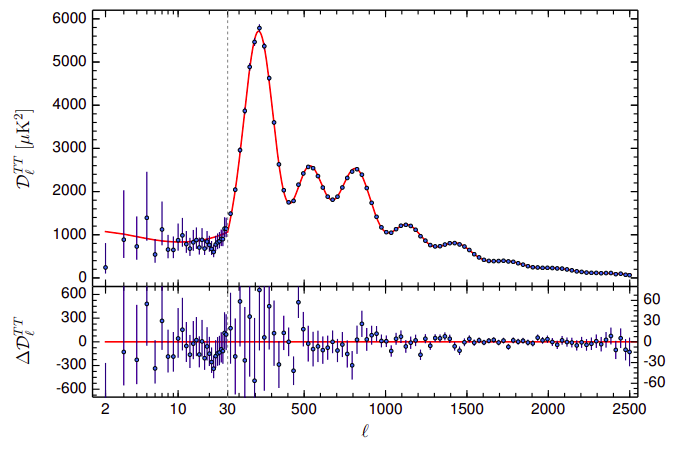
\includegraphics[width=10cm, height=6cm]{figs/PlanckSpectrum.png}
\caption{Power spectrum of the \ac{CMB} obtained by Planck, representing the fluctuations of the temperature of this radiation with respect to the angular angle of observation.}
\label{figure:CMBSpectrum}
\end{center}
\end{figure}

\subsection{Gravitational lensing}

The last evidence supporting the existence of dark matter has been obtained by observing several clusters of galaxies in the Universe, such as the Bullet Cluster, and by studying their mass distribution through gravitational lensing. This effect is a consequence of the general relativity, stating that massive objects lying between distant sources and an observer should act as a lens and bend the light of the object emitted by the source. This deviation of the light is actually proportional to the mass of the object in between the source and the observer, meaning that the gravitational lensing can give us a way to measure the mass distribution within massive objects, such as galaxy clusters.

The bullet Cluster is particularly interesting in this context since it actually provides an evidence for the eventual existence of dark matter which does not rely on any mathematical assumption and cannot at principle be explained by alternate laws of gravitation. Indeed, some observations showed that the spatial deviations between the center of the total mass and the center of the baryonic mass cannot be explained with an alteration of the gravitational force law alone, with a statistical significance of around $8 \sigma$ \cite{BulletClusterSigma}.

\begin{figure}[htbp]
\begin{center}
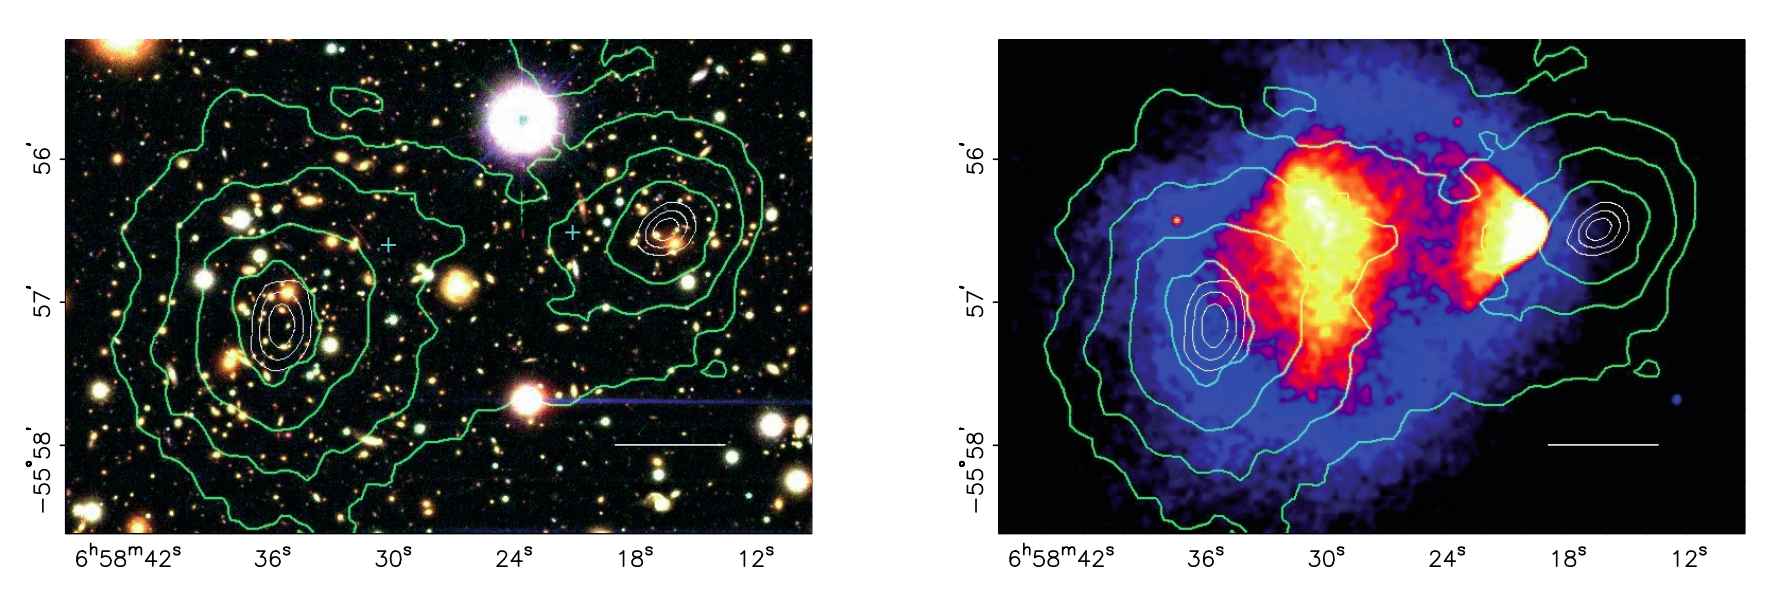
\includegraphics[width=14cm, height=6cm]{figs/BulletCluster.png}
\caption{Mass distributions obtained by the Magellan in the visible (on the left) and Chandra on the X-rays spectrum (on the right) telescopes of the Bullet Cluser, yet another clear evidence for the existence of \ac{DM} \cite{BulletClusterSigma}.}
\label{figure:BulletCluster}
\end{center}
\end{figure}

As seen in Figure~\ref{figure:BulletCluster}, the image taken by Chandra clearly shows an offset between the plasma of the cluster and the actual mass distribution measured through gravitational lensing (green contours).  The mass distribution appears to be slightly deviated compared to what was expected based on the X-ray emissions of this cluster.

\section{Dark matter properties} \label{section:DMProperties}

All the previous observations allow us to list some of the most important properties that the perfect dark matter candidate should have. Even though several theories exist, each giving different properties to the \ac{DM}, we will consider in this work the following mostly accepted properties for such particles:
\begin{itemize}
\item First of all, we will assume that \ac{DM} is a \textbf{particle}. As far as we know, the Universe, is simply composed of particles so there is no objective reason to think that \ac{DM}, being matter with a certain mass, might not be made out of some kind of indivisible particle at some level.
\item First of all, the perfect \ac{DM} candidate should of course be \textbf{dark}. This means that it should not interact at all in with electromagnetic radiation such as light, and that it should therefore be \textbf{electrically neutral}. However, it has to interact gravitationnaly because of the evidences for the evidence of such a particle explained before, mostly relying on gravitational effects.
\item It has to be \textbf{non-baryonic}, mainly because the energy density for the baryonic matter obtained by observing the power spectrum of the \ac{CMB} is too low to account for \ac{DM} as well, as explained in Section~\ref{subsection:CMB}. Indeed, according to these results, baryonic matter account for around 5\% while dark matter accounts for more than 25\% of the energy density of the Universe. 
\item We will also only consider \textbf{cold} dark matter, since the widely accepted $\Lambda CDM$ cosmological model is actually based on this assumption. By cold, we do not refer to the temperature of these particles but actually to their size, and therefore to the velocity by which they can travel in the Universe. Large scale structures of the Universe such as we can observe them today cannot actually not be explained if \ac{DM} is made out of hot/relativistic particles, as represented in Figure~\ref{figure:ColdWarmDM}.
\item It is interesting to report as well that \ac{DM} particles are expected to be found near the electroweak symmetry breaking scale, between \textbf{10 GeV and 1 TeV}. This is a consequence of the expected production mechanism of such particles, the so-called thermal freeze-out. 

This principle tells us that at some point in the history, \ac{DM} was in thermal equilibrium with other primordial standard particles, meaning that its production and annihilation rates were equal. However, because of the expansion of the Universe, at some point \ac{DM} particles were simply too far apart from each other and these reactions maintaining this equilibrium became not efficient enough to maintain this equilibrium. At this stage, the abundance of \ac{DM} became fixed: this is the freeze-out, as represented in Figure~\ref{figure:FreezeOut}.

This principle is interesting because, as a rule of thumb, we can say that if a particle interacts heavily, it will stay longer in equilibrium and its freeze-out abundance will be smaller, so there is a mathematical relation between the strength of the \ac{SM}/\ac{DM} interaction $g$, the mass of the \ac{DM} particle $m_\chi$ and its actual abundance $\Omega_\chi$ that can be measured, as expressed in Equation ~\ref{equation:FreezeOut} \cite{FreezeOut}.
\begin{equation}
\label{equation:FreezeOut}
\Omega_\chi \propto \frac{m_\chi^2}{g^4}
\end{equation}

By using a typical value for $g$ of the order of the Fermi coupling constant $G_0^F \simeq 4.54 \cdot 10^14$ J$^{-2}$, we can see that, in order to observe a freeze-out abundance comparable to the current one, the \ac{DM} candidate should indeed have a mass between 10 GeV and 1 TeV.

\item Finally, they should be \textbf{long-lived}. Indeed, we expect that \ac{DM} particles were produced 13.8 billion years ago during the Big Bang, but it seems that we still see them today. They should then be stable particles, or their lifetime should at least be larger than the age of the Universe itself.
\end{itemize}

\begin{figure}[htbp]
\begin{center}
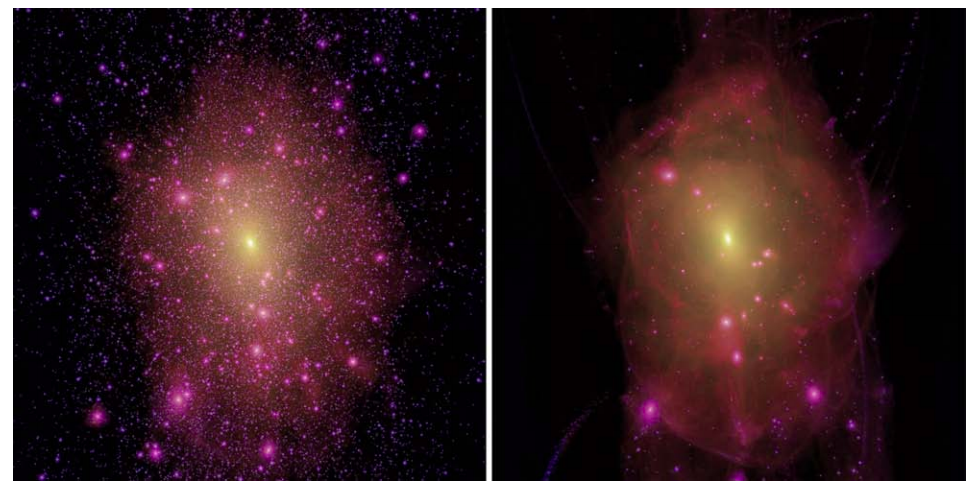
\includegraphics[width=14cm, height=6cm]{figs/ColdWarmDM.png}
\caption{Computer simulations for cold (on the left) and warm (on the right) \ac{DM} scenarios and their impact on a galactic halo at 0 redshift \cite{ColdWarmDM}.}
\label{figure:ColdWarmDM}
\end{center}
\end{figure}

\begin{figure}[htbp]
\begin{center}
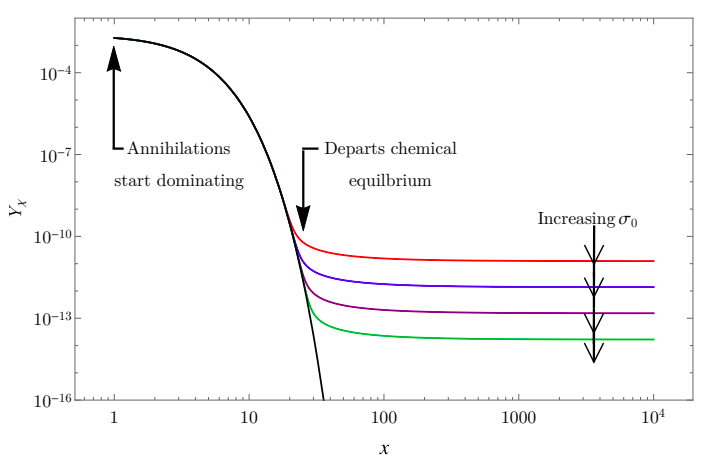
\includegraphics[width=10cm, height=6cm]{figs/FreezeOut.png}
\caption{Schematic representation of the freeze-out process, representing the abundance of a 500 GeV \ac{DM} as $Y_\chi$ with respect to the time and the impact of increasing cross-section values on this freeze-out abundance \cite{FreezeOut2}.}
\label{figure:FreezeOut}
\end{center}
\end{figure}

All these properties narrow quite a lot the number of possible \ac{DM} candidates, as we will see in the following section.

\section{Dark matter candidates} \label{section:DMCandidates}
\section{Dark matter searches} \label{section:DMSearches}
\section{Production at the LHC} \label{section:ourChannel}
\subsection{The single top production channel} \label{subsection:singleTopChannel}
\subsection{The $t \bar t$ production channel} \label{subsection:ttChannel}
\section{Previous results} \label{section:PreviousResults}

\chapter{The experimental device} \label{chapter:Device}
\section{The LHC accelerator}
\section{The CMS detector}
\subsection{Tracker}
\subsection{Electromagnetic calorimeter}
\subsection{Hadronic calorimeter}
\subsection{Muon system}
\subsection{Trigger}
\subsection{Data acquisition}

\chapter{Objects reconstruction} \label{chapter:Reco}
\section{Particle Flow algorithm}
\section{Leptons reconstruction}
\subsection{Electrons}
\subsection{Muons}
\section{Jets reconstruction}
\subsection{B-tagging}
\section{Missing transverse energy}

\chapter{Data, signals and backgrounds} \label{chapter:Samples}
\section{Data samples}
\section{Signal samples}
\section{Background prediction}
\subsection{The main background: $t \bar t$}
\subsubsection{$t \bar t$ reconstruction}
\subsection{Drell-Yan estimation}
\subsection{Non prompt contamination}
\subsection{Smaller backgrounds}
\subsection{Weights and corrections applied}

\chapter{Event selection} \label{chapter:Selection}
\section{Signal regions}
\section{Control regions}
\section{Background-signal discrimination} \label{section:Discrimination}
\subsection{Discriminating variables}
\subsection{Neural network}

\chapter{Results and interpretations} \label{chapter:FinalResults}
\section{Systematics and uncertainties}
\section{Results}

\chapter{Conclusions} \label{chapter:Conclusion}
\section{Future prospects}

\begin{appendices}
  
\end{appendices}

%List of figures
\listoffigures 

%List of tables
\listoftables

\addcontentsline{toc}{chapter}{Bibliography}

\begin{thebibliography}{1}

\bibitem{HiggsPostulate1} 
\href{https://journals.aps.org/prl/abstract/10.1103/PhysRevLett.13.321}{F. Englert and R. Brout, 
"Broken symmetry and the mass of gauge vector mesons",
Phys. Rev. Lett. 13, pp. 321-323, 1964}

\bibitem{HiggsPostulate2} 
\href{https://journals.aps.org/prl/abstract/10.1103/PhysRevLett.13.508}{P. W. Higgs, 
"Broken symmetries and the masses of gauge bosons",
Phys. Rev. Lett. 13, pp. 508-509, 1964}

\bibitem{HiggsDiscovery1} 
\href{https://arxiv.org/abs/1207.7235}{S. Chatrchyan et al.,
"Observation of a new boson at a mass of 125 GeV with the CMS experiment at the LHC",
Phys. Lett. B716, pp. 30-61, 2012}

\bibitem{HiggsDiscovery2} 
\href{https://arxiv.org/abs/1207.7214}{G. Aad et al.,
"Observation of a new particle in the search for the Standard Model Higgs boson with the ATLAS detector at the LHC", 
Phys. Lett. B716, pp. 1-29, 2012}

\bibitem{FirstEvidence}
\href{https://ui.adsabs.harvard.edu/abs/1980ApJ...238..471R/abstract}{V.C. Rubin, W.K. Ford and N. Thonnard,
"Rotational properties of 21 SC galaxies with a large range of luminosities and radii, from NGC 4605 (R=4kpc) to UGC 2885 (R=122kpc)",
Astrophysical Journal 238, pp. 471-487, 1980}

\bibitem{RotationCurves}
\href{https://academic.oup.com/mnras/article/249/3/523/1005565}{K.G. Begeman, A.H. Broeils and R.H. Sanders,
"Extended rotation curves of spiral galaxies - Dark haloes and modified dynamics",
Monthly Notices of the Royal Astronomical Society, vol. 249, issue 3, ISSN 0035-8711, 1991}

\bibitem{BulletCluster}
\href{https://arxiv.org/abs/1605.04307}{A. Robertson, R. Massey and V. EkCMBTemperaturee,
"What does the Bullet Cluster tell us about self-interacting dark matter?",
Monthly Notices of the Royal Astronomical Society, vol. 465, issue 1, 2017}

\bibitem{CMBAnisotropies} 
\href{https://arxiv.org/abs/1804.01092}{J.B. Mu�oz, C. Dvorkin and A. Loeb,
"21-cm Fluctuations from Charged Dark Matter",
Phys. Rev. Lett. 121, 121301 (2018)}

\bibitem{Repartition}
\href{https://arxiv.org/abs/1201.3939}{A. Natarajan,
"A closer look at CMB constraints on WIMP dark matter",
Phys. Rev. D85, 2012}

\bibitem{MFVYukawa}
\href{https://arxiv.org/abs/hep-ph/0207036}{G. D'Ambrosio G.F. Giudice, G. Isidori and A. Strumia,
"Minimal Flavour Violation: an effective field theory approach",
Nucl.Phys. 645, pp 155-187, 2002}

%\bibitem{YukawaMeasurement}
%\href{https://arxiv.org/abs/1907.01590}{CMS Collaboration,
%"Measurement of the top quark Yukawa coupling from $t \bar t$ kinematic distributions in the lepton+jets final state in proton-proton collisions at $\sqrt{s}= 13$ TeV",
%Phys. Rev. D 100, 072007 (2019)}

\bibitem{PDG}
\href{http://pdg.lbl.gov/}{M. Tanabashi et al.,
Particle Data Group,
Phys. Rev. D98, 030001 (2018)}

%\bibitem{PreviousSingleTopAllLep2CDF}
%\href{https://arxiv.org/abs/1202.5653}{CDF Collaboration,
%"Search for a dark matter candidate produced in association with a single top quark in pp collisions at $\sqrt{s} = 1.96$ TeV",
%Phys. Rev. Lett. 108 (2012) 201802} MONOTOP!

\bibitem{PreviousDoubleTopSingleLep8CMS}
\href{https://arxiv.org/abs/1504.03198}{CMS Collaboration,
"Search for the production of dark matter in association with top-quark pairs in the single-lepton final state in proton-proton collisions at $\sqrt{s} = 8$ TeV",
JHEP, vol. 6 121, 2015}

\bibitem{PreviousDoubleTopDiLep8CMS}
\href{http://inspirehep.net/record/1292446}{CMS Collaboration,,
"Search for the Production of Dark Matter in Association with Top Quark Pairs in the Di-lepton Final State in pp collisions at $\sqrt{s} = 8$ TeV",
CMS-PAS-B2G-13-004, 2014}

\bibitem{PreviousDoubleTopAllLep8ATLAS}
\href{https://arxiv.org/abs/1410.4031}{
"Search for dark matter in events with heavy quarks and missing transverse momentum in pp collisions with the ATLAS detector",
Eur. Phys. J. C (2015) 75:92}

%\bibitem{PreviousSingleTopAllLep8ATLAS}
%\href{https://arxiv.org/abs/1410.5404}{ATLAS Collaboration,
%"Search for invisible particles produced in association with single-top-quarks in proton-proton collisions at $\sqrt{s} = 8$ TeV with the ATLAS detector",
%Eur. Phys. J. C (2015) 75:79} MONOTOP!

\bibitem{PreviousDoubleTopNoLep13ATLAS}
\href{http://inspirehep.net/record/1480057}{ATLAS Collaboration,
Search for the Supersymmetric Partner of the Top Quark in the Jets+Emiss Final State at $\sqrt{s} = 13$ TeV",
ATLAS-CONF-2016-077
}

\bibitem{PreviousDoubleTopOneLep13ATLAS}
\href{http://inspirehep.net/record/1480030/}{ATLAS Collaboration,
"Search for top squarks in final states with one isolated lepton, jets, and missing transverse momentum in $\sqrt{s} = 13$ TeV pp collisions with the ATLAS detector",
ATLAS-CONF-2016-050, 2016}

\bibitem{PreviousDoubleTopDiLep13ATLAS}
\href{http://inspirehep.net/record/1480056}{ATLAS Collaboration,
"Search for direct top squark pair production and dark matter production in final states with two leptons in $\sqrt{s} = 13$ TeV pp collisions using 13.3 fb$^{-1}$ of ATLAS data",
ATLAS-CONF-2016-076, 2016}

\bibitem{PreviousDoubleTopBottomAllLep13ATLAS}
\href{https://arxiv.org/abs/1710.11412}{ATLAS Collaboration,
"Search for dark matter produced in association with bottom or top quarks in $\sqrt{s} = 13$ TeV pp collisions with the ATLAS detector",
Eur. Phys. J. C 78 (2018) 18}

\bibitem{PreviousDoubleTopBottomAllLep13CMS}
\href{http://inspirehep.net/record/1603635}{CMS Collaboration,
Search for dark matter produced in association with heavy-flavor quark pairs in proton-proton collisions at $\sqrt{s} = 13$ TeV",
Eur. Phys. J. C (2017) 77: 845}

\bibitem{PreviousDoubleTopAllLep13CMS}
\href{https://arxiv.org/abs/1807.06522}{CMS Collaboration,
"Search for dark matter particles produced in association with a top quark pair at $\sqrt{s} = 13$ TeV",
Phys. Rev. Lett. 122, 011803 (2019)}

\bibitem{PreviousSingleDoubleTopAllLep13CMS}
\href{https://arxiv.org/abs/1901.01553}{CMS Collaboration,
"Search for dark matter produced in association with a single top quark or a top quark pair in proton-proton collisions at $\sqrt{s} = 13$ TeV",
JHEP, vol. 03 141, 2019}

\bibitem{Zwicky} 
\href{http://articles.adsabs.harvard.edu/cgi-bin/nph-iarticle_query?1933AcHPh...6..110Z&amp;data_type=PDF_HIGH&amp;whole_paper=YES&amp;type=PRINTER&amp;filetype=.pdf}{
F. Zwicky,
"Die Rotverschiebung von extragalaktischen Nebeln",
Helvetica Physica Acta , vol. 6, pp. 110-127, 1933}

\bibitem{ZwickyWrong}
\href{https://arxiv.org/pdf/astro-ph/9904251.pdf}{S. Van den Bergh,
"The early history of dark matter",
Dominion Astrophysical Observatory, 1999
}

\bibitem{VeraRubin}
\href{https://ui.adsabs.harvard.edu/abs/1970ApJ...159..379R/abstract}{V.C. Rubin, W.K. Ford,
"Rotation of the Andromeda Nebula from a Spectroscopic Survey of Emission Regions",
Astrophysical Journal 159, p. 379, 1970
}

\bibitem{CMBDiscovery}
\href{https://ui.adsabs.harvard.edu/abs/1965ApJ...142..419P/abstract}{A. A. Penzias, R.W. Wilson,
"A Measurement of Excess Antenna Temperature at 4080 Mc/s",
Astrophysical Journal 142, pp. 419-421
}

\bibitem{CMBTemperature}
\href{https://iopscience.iop.org/article/10.1088/0004-637X/707/2/916}{D.J. Fixsen,
"The temperature of the cosmic microwave background",
Astrophysical Journal, 2009
}

\bibitem{PowerSpectrum}
\href{https://www.roe.ac.uk/ifa/postgrad/pedagogy/2006_tojeiro.pdf}{R. Tojeiro,
"Understanding the Cosmic Microwave Background Temperature Power Spectrum",
2006
}

\bibitem{Planck}
\href{https://arxiv.org/abs/1807.06209}{Planck Collaboration, 
"Planck 2018 results. VI. Cosmological parameters", 2018
}

\bibitem{Constants}
\href{http://pdg.lbl.gov/2019/reviews/rpp2018-rev-astrophysical-constants.pdf}{
"Astrophysical Constants and Parameters", 
2019
}

\bibitem{BulletClusterSigma}
\href{https://iopscience.iop.org/article/10.1086/508162}{D. Clowe et all.,
"A Direct Empirical Proof of the Existence of Dark Matter",
Astrophysical Journal Letters 648, 2006
}

\bibitem{FreezeOut}
\href{https://arxiv.org/pdf/1712.09919.pdf}{K.R. Dienes, J. Fennick, J. Kumar, B. Thomas
"Dynamical Dark Matter from Thermal Freeze-Out",
Phys. Rev. D 97, 063522 (2018)
}

\bibitem{ColdWarmDM}
\href{https://arxiv.org/pdf/1210.0544.pdf}{C.S. Frenk, S.D.M. White,
"Dark matter and cosmic structure",
Annalen der Physik, p. 22 , 2012
}

\bibitem{FreezeOut2}
\href{http://inspirehep.net/record/1683379/files/fulltext.pdf}{R. Kirk,
"Dark matter genesis"}

\end{thebibliography}

\end{document}
